%!TEX root = brainreader.tex

\section{Introduction}
\IEEEPARstart{F}{unctional} magnetic resonance imaging, or fMRI, is a technology used in neuroscientific research for recording brain activity. It can be used for a technique called ``brain decoding'', which refers to identifying sensory stimuli or brain states that an individual is experiencing, based on their brain activity. Researchers have been able to use fMRI data to decode visual stimuli in several fMRI studies (\cite{Kamitani, Naselaris, Nishimoto}).

The most complex reconstruction of visual information to date was done by Nishimoto and colleagues in the Gallant lab at UC Berkeley. The researchers built a forward model predicting fMRI signals in the visual cortex from the structural content in the movies seen by the subject. The structural content was captured by processing the movies with spatiotemporal motion energy filters. These filters represent spatial frequency, temporal frequency, and orientation features at different scales and locations on the screen. 

Ridge regression was used to fit a predictive model between the motion energy parameterization of the movies and the fMRI responses at each recording site (voxel) in the brain. A Bayesian approach was then used to build the inverse model. The posterior probability of the movie decoded from brain activity was estimated by combining a likelihood function given by the forward model and a natural movie prior. In the absence of an explicit distribution of natural images, the natural prior was simulated by sampling 18,000,000 seconds of videos from YouTube.

The model was successful, and using the likelihood of brain activity to identify each timepoint in a held-out stimulus set produced the correct result 95\% of the time. To visualize the result of the direct decoding using the natural movie prior, a set of 100 clips with the highest log likelihood according to the model was selected and averaged. The resulting video can be viewed here (http://www.youtube.com/watch?v=nsjDnYxJ0bo). While the decoding results are quite accurate as seen from the identification, the video appears fuzzy and is misleading about the precision of the decoding. Using computational techniques, we can improve the quality of these output videos (Figure \ref{fig:avg}).


\begin{figure}[t]
\centering
    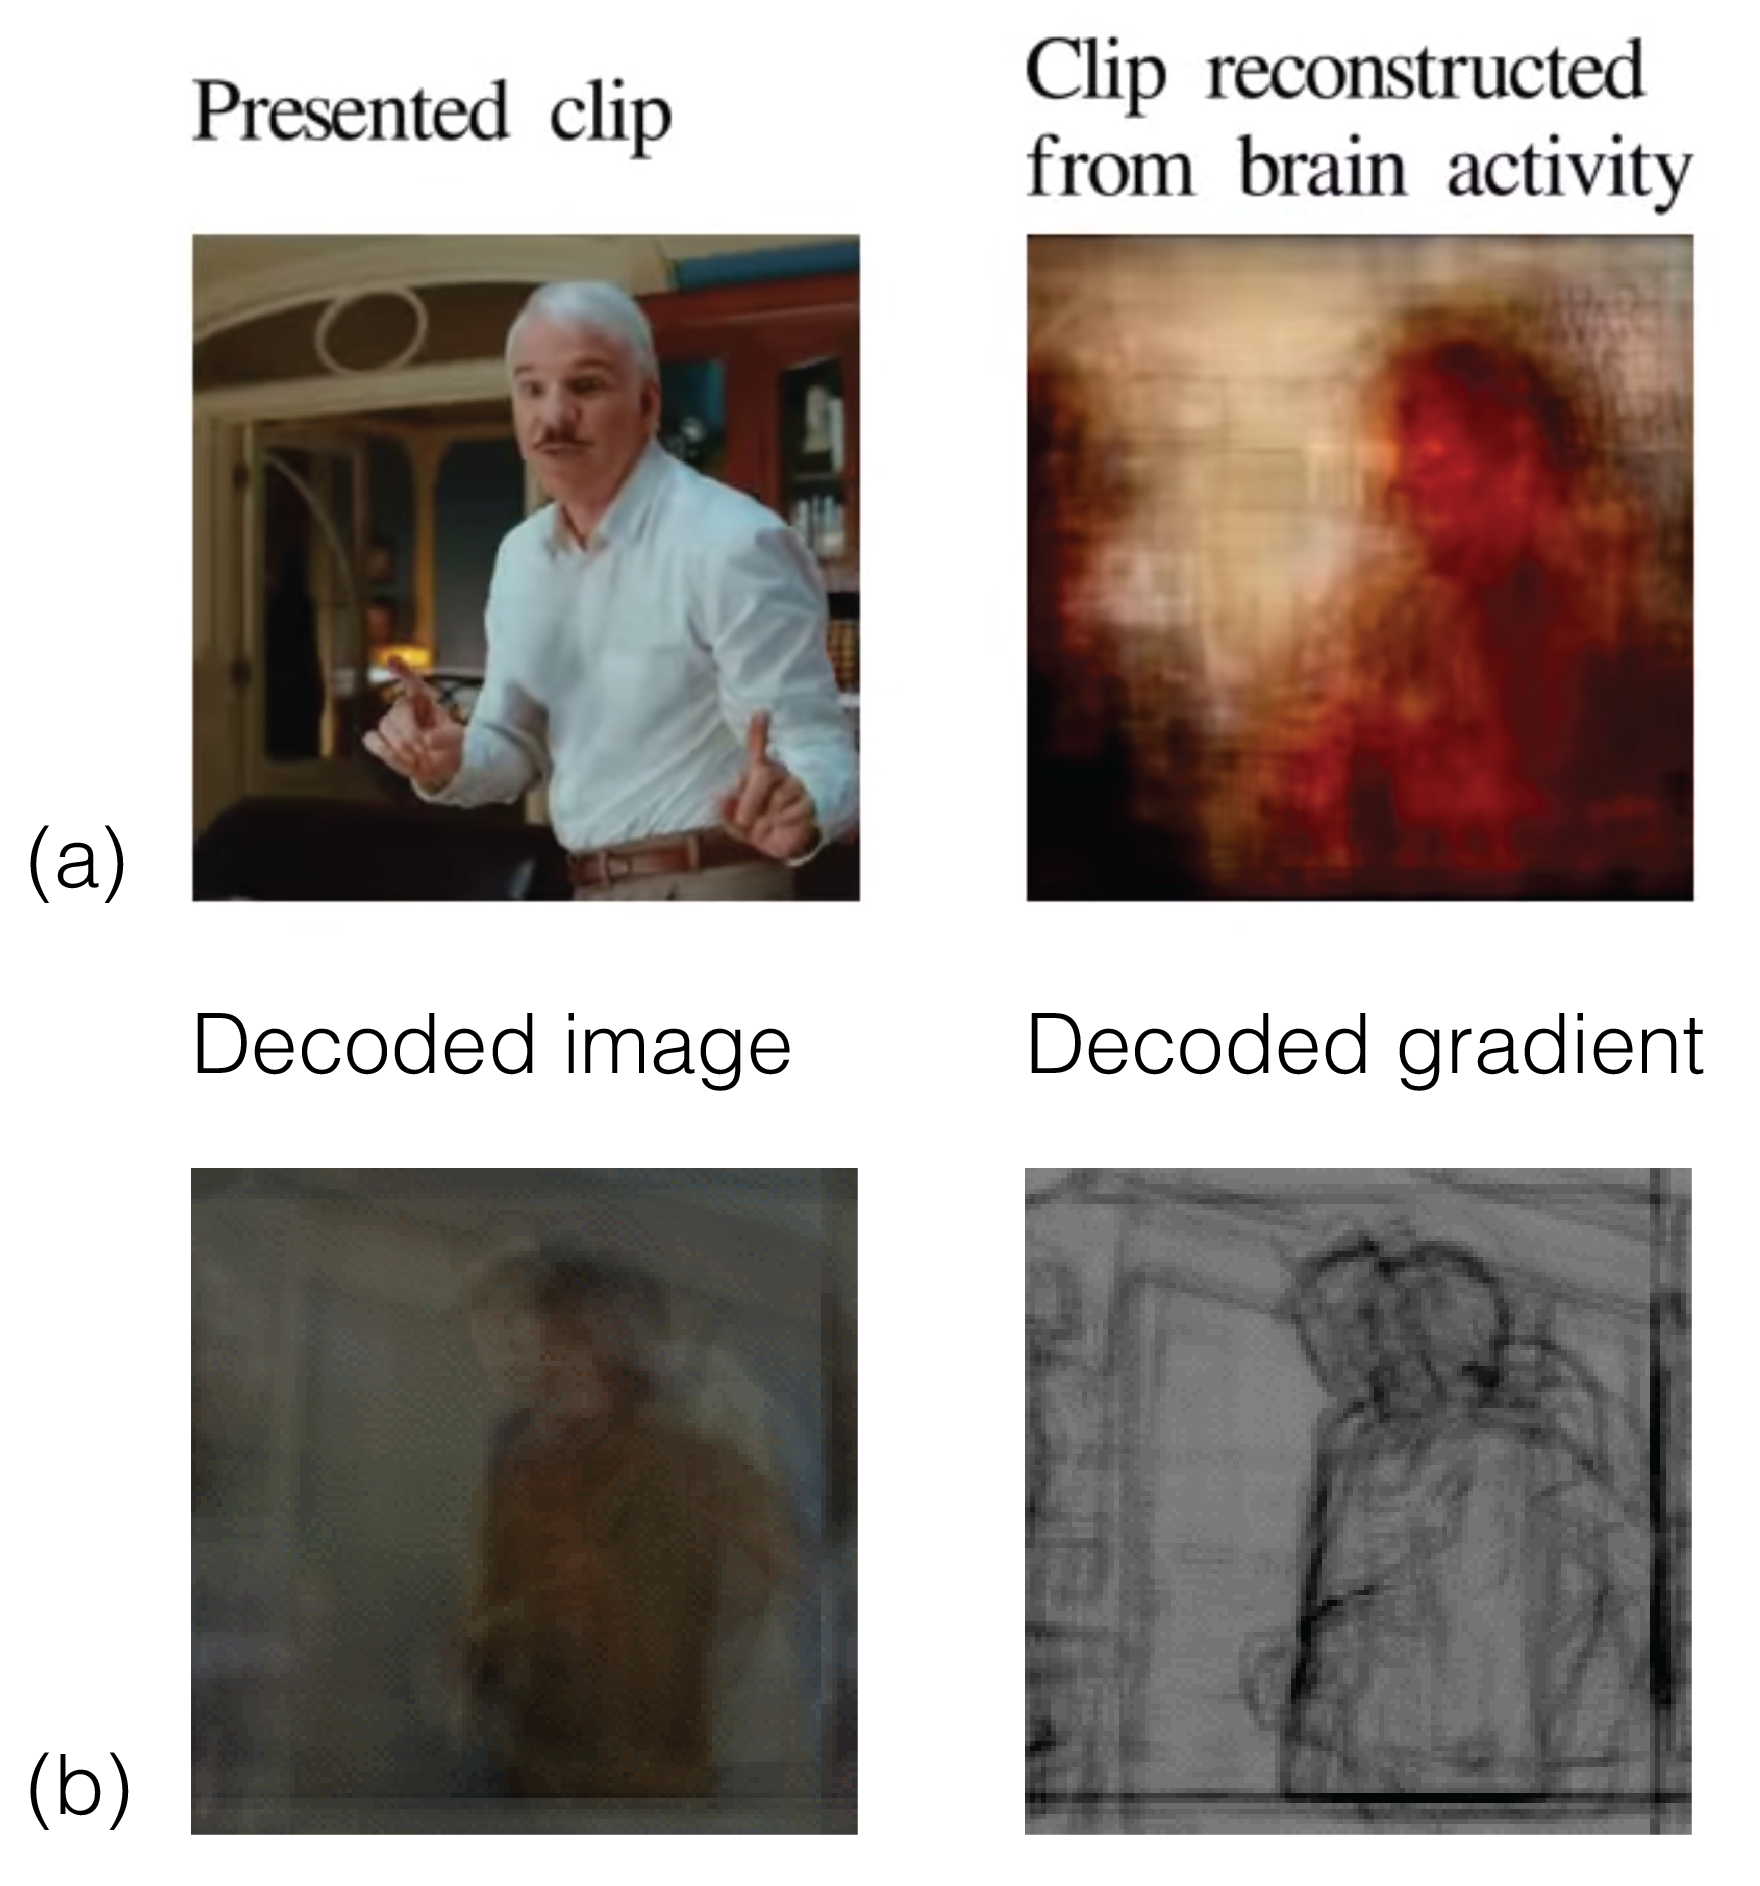
\includegraphics[width=1.0\columnwidth]{figures/fig1B.png}
\caption{a) The first generation of visualization for BrainDreamer clips: the top 100 guesses are simply averaged and overlaid to create an output image at each frame.  This belies the accuracy of the technique, which is quite high. b) Our improved visualization.}
\label{fig:avg}
\end{figure}


Instead of a simple averaging process for turning guesses into an output video, we used several more sophisticated approaches.  First, we simply performed weighted averaging, using relative log likelihood scores of the clips as our weights.  This already constituted an improvement over na\"{i}ve weighting (Figure \ref{fig:weighted}).

\begin{figure}[t]
\centering
    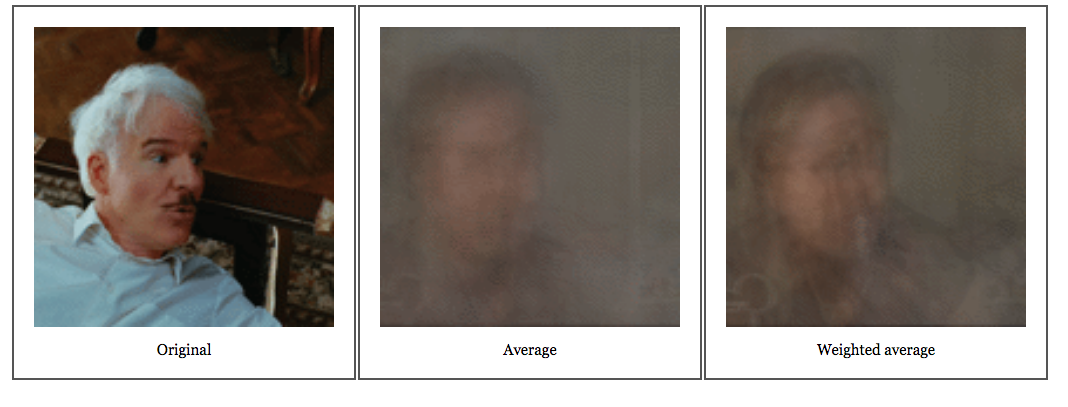
\includegraphics[width=1.0\columnwidth]{figures/orig-avg-weighted.png}
\caption{Using a weighted average improves over the na\"{i}ve average.  Left: original clip presented.  Center: na\"{i}ve average.  Right: weighted average.}
\label{fig:weighted}
\end{figure}


After using weighted averaging, we turned to even more sophisticated techniques: HOG feature alignment and SIFT flow.  These give us additional information on the edges makeup and semantic scene composition of both the original clip and the top 100 guesses as predicted by the original fMRI-based system.  We perform three steps to create our visualization from these ranked guesses: pruning, consistency-assurance, and visual morphing.